\documentclass[../fem.tex]{subfiles}

\begin{document}
\section{Linear Systems}%
\label{sec:linear_systems}

\begin{enumerate}
  \item Issues
  \item Data Structure
    \begin{enumerate}
      \item FULL
      \item INDEX
      \item CSR
    \end{enumerate}
  \item Multiplication
  \item Krylov Subspaces
    \begin{enumerate}
      \item Reasoning
      \item Definition?
    \end{enumerate}
  \item Arnoldi Iteration
  \item GMRES
\end{enumerate}

As the finite element method constructs a global system of equations, we need
to implement a method for solving this system of linear equations. However,
there are issues with the magnitude of this system. Let us take a sample
situation where our mesh has $\sim 100,000$ elements. This would result in a
global matrix of $10,000,000,000$ values, which would require $\sim 80Gb$ of
memory. Solving this matrix using straight forward gaussian elimination, which
has order $\mathcal{O}(n^3)$ time complexity, would require extream amounts of
time and memory to compute. Because of these issues we need to utilize methods
that allow us to avoid these issues that arise in the brute force method of
solving the system of linear equations.

\subsection{Data Structures}%
\label{sub:data_structures}

The first issue that we need to solve is the issue of memory requirements for
the large matricies. We can greatly use that fact that the global matrix will
be a sparse matrix. This is true by the method of construction of our matrix,
most of the elements will be zero.

Using this knowledge we examine three methods of matrix storage. We use a sense
of \textit{efficiency} to impy memory efficiency, and the memory usage required
to store the matrix.

We assume that the indicies of the matrix are stored as
\mintinline{cpp}{uint64_t} which requires $8$ bytes of memory, and that the
values are stored as \mintinline{cpp}{double} which requires $8$ bytes of
memory. We use $N$ to denote the dimenson of the square matrix, and $S$ to
represent the percent of elements that are non zero in the matrix.

\begin{enumerate}[label=\arabic*.]
  \item Full matrix storage.
  \item Dictionary of Keys.
  \item Compressed Row Storage.
\end{enumerate}

\subsubsection{Full Matrix}%
\label{ssub:full_matrix}

This method simply stores a two dimensional array of \mintinline{cpp}{double}
values. This means that the memory requirement will be $N^2\cdot 8$ bytes. Note
that this is independent of the sparicty of the matrix, so even if the matrix
has only one element the memory usage is still the same as a full matrix.

An example of this is the following

\begin{align*}
   A = \begin{bmatrix}
     10 & 0 & 0 & 0 & -2 & 0 \\
     3 & 0 & 0 & 0 & 0 & 3 \\
     0 & 7 & 8 & 7 & 0 & 0 \\
     3 & 0 & 0 & 0 & 5 & 0 \\
     0 & 8 & 0 & 9 & 0 & 13 \\
     0 & 4 & 0 & 0 & 2 & -1
   \end{bmatrix}
\end{align*}

For this method we directly store this matrix into memory saving all of the
zero elements.

This is the most simplistic method for storing a matrix. It will not suffice
for most of our situations, but it is important to have a base line to compare
to, to determin the efficiency of our later methods.

\begin{Figure}
  \begin{center}
    \begin{tikzpicture}[scale=0.8, transform shape]
      \begin{axis}[axis lines=middle, xmin=0.0, xmax=1.0, ymin=0.0, ymax=900.0]
        \addplot[forget plot] {800};
      \end{axis}
    \end{tikzpicture}
  \end{center}
  \captionof{figure}{Memory usage for full matrix storage at different
  percentages of sparicty.}
  \label{fig:mat_full}
\end{Figure}

\subsubsection{Dictionary of Keys}%
\label{ssub:dictionary_of_keys}

The next logical step for improving our matrix efficiency, is to only store the
elements that are not zero. A simple way of doing this is to store the
\textit{row} and \textit{column} indecies and the associated value at that
point. This means that for each value we store three numbers, but we only store
the values that are not zero. This means that this is only effective to an
extent, as a full matrix would require three times the memory of the method in
section \ref{ssub:full_matrix}.

Using the same example from above

\begin{align*}
   A = \begin{bmatrix}
     10 & 0 & 0 & 0 & -2 & 0 \\
     3 & 0 & 0 & 0 & 0 & 3 \\
     0 & 7 & 8 & 7 & 0 & 0 \\
     3 & 0 & 0 & 0 & 5 & 0 \\
     0 & 8 & 0 & 9 & 0 & 13 \\
     0 & 4 & 0 & 0 & 2 & -1
   \end{bmatrix},
\end{align*}

we implement the DOK method for sparse matrix storage.

\begin{align*}
  A = \begin{bmatrix}
    0 & 0 & 10 \\
    0 & 4 & -2 \\
    1 & 0 & 3 \\
    1 & 5 & 3 \\
    2 & 1 & 7 \\
    2 & 2 & 8 \\
    2 & 3 & 7 \\
    3 & 0 & 3 \\
    3 & 4 & 5 \\
    4 & 1 & 8 \\
    4 & 3 & 9 \\
    4 & 5 & 13 \\
    5 & 1 & 3 \\
    5 & 4 & 2 \\
    5 & 5 & -1
  \end{bmatrix}
\end{align*}

Where the first column in the row index ($0$ based), the second column in the
column index ($0$ based), and the third column is the value stored at that
position.

We find that this method requires $SN^2\cdot24$ bytes. It is clear to see that
if $S$ is large, then this method is significantly less effective but if $S$ is
small enough, then there is additional efficiency to be gained. We can compute
the minimum value of $S$ that would allow for increased efficiency like so

\begin{align*}
  SN^2\cdot24&=N^2\cdot8\\
  S&=\frac{8}{24}\\
  S&=\frac{1}{3}.
\end{align*}

Thus for any matrix where more than a third of its elements not zero, means
that we would be better off using a full matrix storage system.

\begin{Figure}
  \begin{center}
    \begin{tikzpicture}[scale=0.8, transform shape]
      \begin{axis}[axis lines=middle, xmin=0.0, xmax=1.0, ymin=0.0]
        \addplot[forget plot] {800};
        \addplot[forget plot] {x*2400};
      \end{axis}
    \end{tikzpicture}
  \end{center}
  \captionof{figure}{Memory usage for DOK at different percentages of
  sparicty.}
  \label{fig:mat_dok}
\end{Figure}

\subsubsection{Compressed Row Storage}%
\label{ssub:compressed_row_storage}

This method take the concept of DOK, and modifies it by the realization that
many elements will be on the same row, so we just need to store the number of
elements in a row, the elements column index, and the value. This means that
for every value, we now only need to store two numbers, and we have a list of
row counts that must exists for all number of non-zero elements.

A slight optimization that we introduce, is instead of storing the number of
elements in each row, we store the total number of elements so far. This is a
slight improvement in the coputational implementation for element access.

This means that for every matrix, we need to store three vectors.
\mintinline{cpp}{val}, \mintinline{cpp}{col_ind}, and
\mintinline{cpp}{row_ptr}.

Using our example matrix,

\begin{align*}
   A = \begin{bmatrix}
     10 & 0 & 0 & 0 & -2 & 0 \\
     3 & 0 & 0 & 0 & 0 & 3 \\
     0 & 7 & 8 & 7 & 0 & 0 \\
     3 & 0 & 0 & 0 & 5 & 0 \\
     0 & 8 & 0 & 9 & 0 & 13 \\
     0 & 4 & 0 & 0 & 2 & -1
   \end{bmatrix},
\end{align*}

we find our three vectors to be

\begin{align*}
  \text{\mintinline{cpp}{row_ptr}} &= \left[0,2,4,7,8,12,15\right]\\
  \text{\mintinline{cpp}{col_ind}} &= \left[\ \;0,\ \ 4,0,5,1,2,3,0,4,1,3,\ \;5,1,4,\ \ 5\right]\\
  \text{\mintinline{cpp}{val}} &= \left[10,-2,3,3,7,8,7,3,5,8,9,13,4,2,-1\right]
\end{align*}

Note that we can easily find the number of nonzero elements by reading the last
value in \mintinline{cpp}{row_ptr}.

We can find the efficiency of this method of matrix storage to be
$8N+SN^2\cdot16$. Again it is clear that if the matrix is full, then this
method is incredibly inefficient. It is also intresting to note that if the
matrix is empty, then the DOK method is more efficient. There are two values of
$S$ where

\begin{enumerate}[label=\arabic*.]
  \item Dictionary of keys transitions from being more efficent to less.
  \item Full matrix transitions from being less efficient to more.
\end{enumerate}

We solve for both of these values of $S$. First, for when DOK becomes less
efficient than CRS.

\begin{align*}
  8N+SN^2\cdot16&=SN^2\cdot24\\
  8N&=8SN^2\\
  S&=\frac{1}{N}.
\end{align*}

And when the full matrix becomes more efficent.

\begin{align*}
  8N+SN^2\cdot16&=N^2\cdot8\\
  16SN^2&=8N^2-8N\\
  S&=\frac{N-1}{2N}
\end{align*}

It is intresting to take notice that the range in which this method is most
efficient is dependent on the size of our matrix. Thus we only want to use this
value when

\begin{align*}
  \frac{1}{N}<S<\frac{N-1}{2N}.
\end{align*}

Using this relation we can construct a plot for the range of $S$ values in
relation of $N$ inwhich this method should be utilized.

\gtodo{Add filled plot of range of optimal $S$ for given $N$. It looks really
cool.}

We can use this relation to see that for large $N$, this method is the most
efficent between

\begin{align*}
   0 < S < 0.5
\end{align*}

Because of this asymptotic approch of this range of sparcity for maximum
efficiency, we use this method of sparse matrix storeage in our implementation.

\begin{Figure}
  \begin{center}
    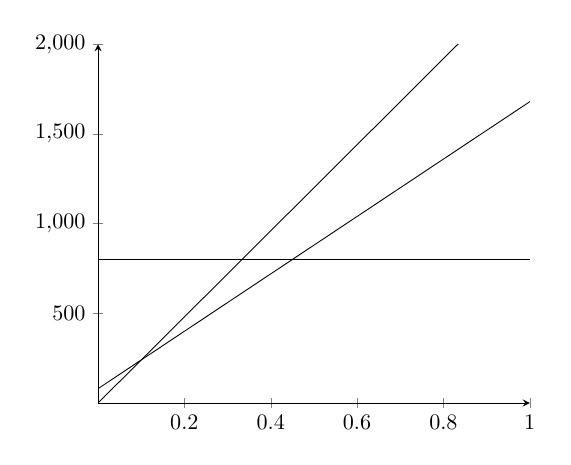
\begin{tikzpicture}[scale=0.8, transform shape]
      \begin{axis}[axis lines=middle, xmin=0.0, xmax=1.0, ymin=0.0]
        \addplot[forget plot] {800};
        \addplot[forget plot] {x*2400};
        \addplot[forget plot] {80+x*1600};
      \end{axis}
    \end{tikzpicture}
  \end{center}
  \captionof{figure}{Memory usage for CRS and DOK at different percentages of
  sparicty.}
  \label{fig:mat_CRS}
\end{Figure}

\subsubsection{Vectors}%
\label{ssub:vectors}

We will simmilarly have large vectors, and can implement a similar method for
sparse vector storage, but this would be counter productive, as our large
vectors are not likly to be sparse. Thus using a sparce represetnation of a
vector would actualy consume more memory than the full vector storage method.

\end{document}
